\section{Hybrid SVD + Windowed Multipole}
\label{sec:hybrid}

\subsection{Memory of the representation (narrow claim)}
\label{sec:hybrid_mem}

We read the MIT ENDF/B-VII.1 WMP library and measure the
on-disk and in-memory payload per nuclide, with SVD rank-$2$
coverage of the smooth remainder.
Table~\ref{tab:hybrid_mem} reports per-nuclide totals; script
\texttt{scripts/hybrid\_svd\_wmp\_experiment.py}, raw output
\texttt{outputs/hybrid\_wmp/results.txt}.

\begin{table}[htb]
\centering
\caption{Representation-byte accounting for WMP vs four
reaction channels of a six-temperature pointwise table. This
is a specific narrow comparison; see
Sec.~\ref{sec:hybrid_mem_engine} for the in-engine measurement.}
\label{tab:hybrid_mem}
\begin{tabular}{@{}lrrrrrr@{}}
\toprule
nuclide & WMP range (eV) & WMP disk & WMP payload & pw full (4 rxn × 6 T) & SVD $k{=}2$ smooth & ratio \\
\midrule
U-$234$  & $0$--$1\,500$         & $34.9$~KB  & $28.0$~KB   & $10.2$~MB  & $12.1$~KB  & $260.0\times$ \\
U-$235$  & $0$--$2\,250$         & $567.3$~KB & $559.1$~KB  & $53.7$~MB  & $10.0$~KB  & $96.6\times$ \\
U-$238$  & $0$--$20\,000$        & $603.0$~KB & $594.7$~KB  & $100.1$~MB & $10.7$~KB  & $169.2\times$ \\
O-$16$   & $0$--$2.36\cdot 10^6$ & $38.5$~KB  & $30.8$~KB   & $0.78$~MB  & $53.3$~KB  & $9.5\times$ \\
H-$1$    & $0$--$2\cdot 10^7$    & $13.7$~KB  & $8.2$~KB    & $155$~KB   & $0.1$~KB   & $18.5\times$ \\
Zr-$90$  & $0$--$53\,500$        & $9.8$~KB   & $4.9$~KB    & $1.48$~MB  & $4.7$~KB   & $156.9\times$ \\
Zr-$91$  & $0$--$10\,000$        & $16.8$~KB  & $9.5$~KB    & $3.17$~MB  & $4.8$~KB   & $227.7\times$ \\
Zr-$92$  & $0$--$71\,000$        & $21.1$~KB  & $14.2$~KB   & $3.97$~MB  & $4.5$~KB   & $217.3\times$ \\
Zr-$94$  & $0$--$90\,000$        & $20.7$~KB  & $14.2$~KB   & $4.22$~MB  & $5.2$~KB   & $222.8\times$ \\
\midrule
\textbf{total} & --- & $1.30$~MB & $1.23$~MB & $\mathbf{177.7}$~\textbf{MB} & $0.10$~MB & $\mathbf{132.9\times}$ \\
\bottomrule
\end{tabular}
\end{table}

\textbf{Interpretation, and what the $132.9\times$ does and
does not mean.} This table compares two specific data layouts:
WMP + rank-$2$ SVD-smooth against a six-temperature pointwise
table, both restricted to four reactions
($\sigma_\text{el}, \sigma_\text{t}, \sigma_\text{f},
\sigma_\text{cap}$). It is a \emph{representation}-level
statement about the density of the WMP encoding for the
resolved resonance cross sections of these specific nuclides.
The $132.9\times$ is therefore the density gap between the
WMP encoding and a four-channel pointwise table on the
matching nuclide set; it is not the reduction a transport
engine carrying the full reaction set would see. The
engine-scale measurement is in
Sec.~\ref{sec:hybrid_mem_engine}.

\subsection{WMP vs HDF5 accuracy}
\label{sec:hybrid_acc}

We evaluate WMP on a $20\,000$-point log-spaced grid inside
each $[E_\text{min}^\text{WMP}, E_\text{max}^\text{WMP}]$ at
$T = 294$~K and compare to the HDF5 pointwise reference.

\begin{table}[htb]
\centering
\caption{WMP-vs-pointwise relative error, $T = 294$~K,
$20\,000$ log-spaced points per nuclide.}
\label{tab:hybrid_acc}
\begin{tabular}{@{}lcccccc@{}}
\toprule
 & \multicolumn{3}{c}{Elastic} & \multicolumn{3}{c}{Absorption} \\
\cmidrule(lr){2-4}\cmidrule(lr){5-7}
nuclide & $p_{50}$ & $p_{99}$ & max & $p_{50}$ & $p_{99}$ & max \\
\midrule
U-$234$ & $5.0 \cdot 10^{-5}$ & $1.3 \cdot 10^{-3}$ & $1.6 \cdot 10^{-1}$
        & $8.6 \cdot 10^{-4}$ & $6.7 \cdot 10^{-2}$ & $0.99$ \\
U-$235$ & $5.4 \cdot 10^{-5}$ & $1.2 \cdot 10^{-3}$ & $8.0 \cdot 10^{-2}$
        & $1.9 \cdot 10^{-4}$ & $1.1 \cdot 10^{-3}$ & $9.1 \cdot 10^{-3}$ \\
U-$238$ & $3.9 \cdot 10^{-5}$ & $1.3 \cdot 10^{-3}$ & $6.8 \cdot 10^{-1}$
        & $2.2 \cdot 10^{-4}$ & $8.0 \cdot 10^{-3}$ & $0.88$ \\
O-$16$  & $5.9 \cdot 10^{-5}$ & $3.3 \cdot 10^{-3}$ & $2.4 \cdot 10^{-2}$
        & $3.0 \cdot 10^{-4}$ & $1.4 \cdot 10^{-2}$ & $2.0 \cdot 10^{-2}$ \\
H-$1$   & $4.9 \cdot 10^{-5}$ & $1.3 \cdot 10^{-3}$ & $3.1 \cdot 10^{-3}$
        & $2.2 \cdot 10^{-4}$ & $3.7 \cdot 10^{-3}$ & $8.8 \cdot 10^{-3}$ \\
Zr-$90$ & $5.5 \cdot 10^{-5}$ & $6.7 \cdot 10^{-4}$ & $7.3 \cdot 10^{-2}$
        & $2.9 \cdot 10^{-4}$ & $8.0 \cdot 10^{-3}$ & $4.5 \cdot 10^{-1}$ \\
Zr-$91$ & $2.5 \cdot 10^{-4}$ & $8.8 \cdot 10^{-4}$ & $2.2 \cdot 10^{-2}$
        & $1.9 \cdot 10^{-4}$ & $3.5 \cdot 10^{-2}$ & $2.9 \cdot 10^{-1}$ \\
Zr-$92$ & $2.6 \cdot 10^{-4}$ & $8.9 \cdot 10^{-4}$ & $1.3 \cdot 10^{-1}$
        & $3.3 \cdot 10^{-4}$ & $8.0 \cdot 10^{-3}$ & $0.99$ \\
Zr-$94$ & $8.1 \cdot 10^{-5}$ & $7.4 \cdot 10^{-4}$ & $1.1 \cdot 10^{-1}$
        & $2.9 \cdot 10^{-4}$ & $8.6 \cdot 10^{-3}$ & $0.90$ \\
\bottomrule
\end{tabular}
\end{table}

Median agreement is $\sim\!10^{-4}$, $p_{99}$ is
$\sim\!10^{-3}$. Maximum absolute errors tail to
$10^{-1}$--$10^{0}$ at isolated points for some nuclides
(HDF5 grid samples a narrow peak densely while WMP
evaluation lies a fraction of the peak width away). These do
not carry through to integrated quantities.

\subsection{End-to-end hybrid engine}
\label{sec:hybrid_e2e}

We implemented \texttt{src/wmp.rs} (CPU WMP reader and
Humlicek W4 evaluator) and \texttt{src/transport/hybrid\_xs.rs}
which wraps \texttt{SvdXsProvider}. For each nuclide with WMP
coverage and each energy in
$[E_\text{min}^\text{WMP}, E_\text{max}^\text{WMP}]$, the
hybrid provider substitutes WMP-evaluated elastic, fission,
and capture into the \texttt{MicroXs} returned by the SVD
provider; inelastic, $(n,2n)$, $(n,3n)$ remain on the SVD
path. URR overrides are short-circuited inside the WMP window.

\paragraph{Unit-level validation.}
The CPU WMP evaluator matches
\texttt{openmc.data.\-WindowedMultipole.\_\_call\_\_} to
$\leq 4\cdot 10^{-6}$ relative error on the three dominant
U-$238$ resonances at $T = 293.6$~K
(\texttt{rust\_prototype/src/bin/wmp\_validate.rs}):

\begin{center}
\begin{tabular}{@{}rrrr@{}}
\toprule
$E$ (eV) & OpenMC $\sigma_\text{abs}$ (b) & Rust $\sigma_\text{abs}$ (b) & $\Delta$ rel \\
\midrule
$6.674$  & $7108.719$ & $7108.695$ & $3.3 \cdot 10^{-6}$ \\
$20.9$   & $6352.230$ & $6352.212$ & $2.8 \cdot 10^{-6}$ \\
$36.7$   & $5357.922$ & $5357.903$ & $3.6 \cdot 10^{-6}$ \\
\bottomrule
\end{tabular}
\end{center}

\paragraph{End-to-end $k_\infty$ and throughput.}
Five seeds, $100$ batches ($20$ inactive), $20\,000$
particles per batch on the large-L3 system
(Ryzen~$9800$X3D). The
hybrid row uses the pre-correction sampler (the sampling
fixes of Sec.~\ref{sec:offset} landed after the hybrid
benchmark was complete and a re-run has not been performed);
for the correctness comparison we pair it against the matched
pre-correction CPU SVD rank-$5$ baseline from the same
software revision. The post-correction CPU SVD
rank-$5$ value ($1.32745 \pm 0.00057$,
Table~\ref{tab:keff_pwr_desktop}) is reported for reference.

\begin{table}[htb]
\centering
\caption{End-to-end hybrid SVD+WMP benchmark on PWR pin
cell, large-L3 system (Ryzen~$9800$X3D). Both rows use the
pre-correction sampler so that the hybrid-vs-SVD delta is
measured at matched physics.}
\label{tab:hybrid_endtoend}
\begin{tabular}{@{}lrrrrrr@{}}
\toprule
mode & rank & $k_\infty$ & $\sigma_\text{seed}$ &
$\Delta$ CPU-SVD (pcm) & ns/p & seeds \\
\midrule
CPU SVD (pre-correction, matched)       & $5$ & $1.32643$ & $0.00065$ & $+0$ (ref) & $16\,052$ & $10$ \\
\textbf{Hybrid SVD+WMP (pre-correction)} & $5$ & $\mathbf{1.32557}$ &
 $\mathbf{0.00070}$ & $\mathbf{-86}$ & $\mathbf{33\,051}$ & $5$ \\
\midrule
CPU SVD (post-correction, reference)    & $5$ & $1.32745$ & $0.00057$ & ---        & $15\,511$ & $10$ \\
\bottomrule
\end{tabular}
\end{table}

The hybrid $k_\infty$ is within $86$~pcm of the matched
pre-correction CPU SVD rank-$5$
($\approx 2.3\,\mathrm{SEM}_\text{combined}$): WMP represents
the resonance cross section by a rational pole fit rather
than a piecewise-linear-in-log-log sampling of the same
evaluated-nuclear-data curve, so small systematic
disagreements in the RRR accumulate into a
$\sim\!86$~pcm shift. Provider parity to within two
$\mathrm{SEM}$ at matched physics is the correctness
statement here. Against the post-correction CPU SVD
baseline the raw offset grows to $-188$~pcm, but that
number mixes the hybrid-vs-SVD representation gap with the
angular/fission-energy sampler change; we do not read it as
a representation claim.

Throughput: the hybrid runs at $33\,051$~ns/p, $2.06\times$
slower than CPU SVD rank-$5$. A single WMP lookup on this
hardware is $\sim\!67$~ns against $\sim\!5$~ns for SVD,
and $\sim\!20\%$ of lookups fall in the RRR, so the
ratio is in line with the per-lookup cost inflation.
WMP is a memory-centric representation, and in this engine
it costs throughput.

\subsection{Memory in the actual engine (broad claim)}
\label{sec:hybrid_mem_engine}

\texttt{HybridSvdWmpXsProvider::memory\_report} introspects
the loaded kernels at run time. We report four variants for
the nine-nuclide PWR set at rank-$5$: the pointwise-table
baseline, pure SVD rank-$5$ (all reactions compressed), the
hybrid current state (SVD basis plus WMP payload), and a
smooth-only projection in which the elastic, fission, and
capture SVD kernels are hypothetically rebuilt on the energy
points outside each nuclide's WMP window (a rebuild we have
not implemented because the shared energy grid across
reactions complicates it).

\begin{center}
\begin{tabular}{@{}lrr@{}}
\toprule
 & bytes (MB) & vs pointwise \\
\midrule
Pointwise-table baseline (Sec.~\ref{sec:pwr}) & $101.5$ & $1.0\times$ \\
Pure SVD rank-$5$ (all reactions) & $\sim\!517.9$ & $5.1\times$ \emph{larger} \\
Current hybrid in-solver (SVD basis + WMP payload) & $519.0$ & $5.1\times$ \emph{larger} \\
Smooth-only projection (EFC SVD restricted + WMP) & $487.6$ & $4.8\times$ \emph{larger} \\
\bottomrule
\end{tabular}
\end{center}

\paragraph{Where the bytes actually live.} The dominant
contribution in every SVD-based variant is the discrete
inelastic-level cascade: $41$ MT$=51$--$91$ levels per
uranium nuclide, $10$--$13$ per zircaloy isotope, each
carried as its own rank-$5$ SVD kernel. On the GPU that
cascade alone measures $251.3$~MB --- by itself
$2.5\times$ the entire pointwise-table engine. The
smooth-channel SVD bases (elastic, fission, capture, total
inelastic, $(n,2n)$, $(n,3n)$) together measure
$64.6$~MB; the WMP payload is $1.23$~MB. So switching the
resonance representation to WMP costs essentially zero
memory, and the hybrid-vs-pure-SVD difference is a $6\%$
rounding error. The engine-scale penalty against the
pointwise table is not caused by WMP and is not relieved by
it; it is caused by storing the discrete-level cascade as
per-level rank-$5$ bases rather than per-level scalar
arrays.

\paragraph{Where the representation-byte ratio still applies.}
Equation~\ref{eq:svd_pt_ratio} from
Sec.~\ref{sec:svd_tradeoff} says the SVD-vs-pointwise memory
ratio is $k/T$ for a single reaction. The engine-scale
penalty reported above is not a counter-example: our
pointwise-table baseline is built at a single effective
temperature per material region (one temperature per
nuclide-in-material). In a multi-temperature library
($T = 6$ in the HDF5 files shipped for depletion
feedback), the pointwise baseline would grow to
$\sim\!600$~MB on the same nuclide set while pure SVD and
hybrid stay at $\sim\!519$~MB; the ordering would then
invert. The engine-scale loss we report is therefore a
loss at $T = 1$, not a universal property.

\begin{figure}[htb]
\centering
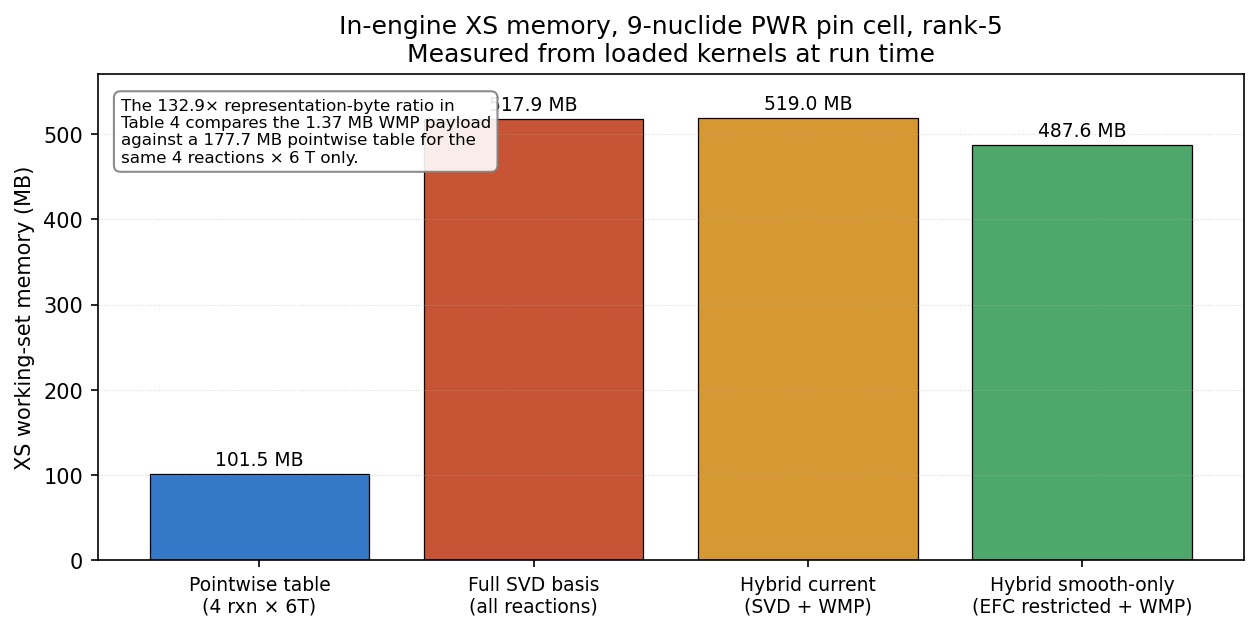
\includegraphics[width=0.82\textwidth]{../outputs/pareto/memory_compare.png}
\caption{In-engine XS working-set memory for the nine-nuclide
PWR pin cell, rank-$5$, measured from live data at run time.
Both hybrid variants carry more memory than the pointwise
table baseline because the SVD kernels for the discrete
inelastic levels, not covered by WMP, dominate the working
set. The $132.9\times$ representation-byte ratio of
Table~\ref{tab:hybrid_mem} is for a different comparison
($1.37$~MB WMP vs $177.7$~MB four-channel pointwise).}
\label{fig:memory_compare}
\end{figure}

The hybrid engine is $4.8$--$5.1\times$ \emph{larger} than
the pointwise-table baseline, because SVD kernels for the
$41$ discrete levels per U nuclide and $10$--$13$ per Zr
isotope dominate memory, and those reactions are not covered
by the public WMP library. The smooth-only restriction
($1.06\times$) is essentially a rounding error.

The $132.9\times$ ratio in Table~\ref{tab:hybrid_mem} is a
correct and reproducible \emph{representation}-byte
comparison --- WMP is denser than a four-channel pointwise
table at matched energy range. But in a transport engine that
carries the full reaction set, WMP does not shrink the
working set unless the rest of the reaction set is also
compressed. A version of this hybrid that achieved
representation-scale memory reduction would need: (i) WMP
coverage for the discrete inelastic cascade
(MT$=51$--$91$); or (ii) a different representation for the
cascade (e.g.\ ENDF-6 nuclear-temperature evaporation
parameters) that is denser than per-level SVD kernels; or
(iii) rebuilding the SVD energy grid to be smooth-only for
\emph{all} reactions, and using a separate table or
analytical evaluation inside the RRR for every reaction. None
of these is implemented here.

\paragraph{So why do the hybrid at all?}
The positive uses we can defend from what we measured:
(a)~WMP is the correct analytical representation for the RRR
and our evaluator is the first pure-Rust implementation we
are aware of (matches OpenMC Python at $\sim\!10^{-6}$
relative error, CUDA port matches to machine precision);
(b)~end-to-end $k_\infty$ agrees with the full-SVD engine to
within two $\mathrm{SEM}$, so the hybrid is \emph{correct}
on this benchmark; (c)~for a future full-core engine where
the cascade reactions are stored more densely than per-level
SVD (e.g. nuclear-temperature evaporation), the RRR saving
becomes proportionally more valuable. We report the hybrid
as a correctness deliverable and as scaffolding for those
future improvements, not as a memory or throughput win on
the present engine.

%% ============================================================
